\documentclass[titlepage]{article}

\usepackage[hidelinks]{hyperref}
\usepackage[table]{xcolor}
\usepackage[english]{babel}
\usepackage{tabularx}
\usepackage[toc,page]{appendix}
\setcounter{secnumdepth}{5}
\usepackage{tikz}
\usepackage{enumitem}
\usepackage{pdfpages}
\usepackage{graphicx}
\usepackage{indentfirst} 
\usepackage{changepage}

%
\usetikzlibrary{arrows, trees, positioning, fit, calc, shadows.blur, shapes.symbols}

\usepackage[top=1.5in, bottom=1.5in, left=2in, right=2in]{geometry}

\def\getfirstword#1{%
    \begingroup
    \edef\@tempa{#1\space}%
    \expandafter\endgroup
    \expandafter\readwords\@tempa\relax
}
\def\readwords#1 #2\relax{%
      \doword{#1}%  #1 = substr, #2 = rest of string
}
\def\doword#1{#1}
\def\endtestwords{}

\newcommand{\myparagraph}[1]{\paragraph{#1}\mbox{}\\}

\addtolength{\oddsidemargin}{-.875in}
\addtolength{\evensidemargin}{-.875in}
\addtolength{\textwidth}{1.75in}

\def \RoCM {Rotation Curve Modeler}
\def \SOCM {Scholarly Observed Celestial Measurements}
\def \RoCS {Rotation Curve Simulation}

\begin{document}

\title{
\textbf{
Software Design Document}
\protect\\
for the
\protect\\
\textbf{
\RoCM\ (RoCM)}
\protect\\
{\small Version 2.0}}

\author{Robert Moss, Alex Clement}
\maketitle

\newpage
\tableofcontents{} 
\newpage

\section{Introduction}

\subsection{Purpose}
The Software Design Document (SDD) is intended to describe the software components of the Rotation Curve Modeler (RoCM). The SDD will include details about the software implementation, the data handling, and the overall design. 

\subsection{Scope}
\begin{enumerate}
	\item Rotation Curve Modeler
	
  \begin{enumerate}	 	
    \item Interact with SOCM (Scholarly Observed Celestial Measurements)
	\begin{enumerate}
		\item Use the repository of observable galactic data to model hundreds/thousands of different galaxies.
	\end{enumerate}
    \item Interact with RoCS (Rotation Curve Simulation)
	\begin{enumerate}
		\item RoCS visualizes the spin of star clusters around the center of a galaxy. 
		\item Include scale and legend for the visualization.
	\end{enumerate}
    \item Allow users to locally import and run their own model (via JavaScript code)
	\begin{enumerate}
		\item Following the defined v(R) input/output standard.
		\item Observable galactic parameters from SOCM will be available as constants.
		\item User defined constants will need to be implemented in the user's function.
	\end{enumerate}
    \item Locally import LaTeX equation for each model (optional)
	\begin{enumerate}
		\item The user can import their own LaTeX equation to be displayed during the data plotting.
		\item Aids in understanding the behavior of each parameter.
	\end{enumerate}
	\item Dynamic parameter sliders
	\begin{enumerate}
		\item For every parameter in the individual models, a dynamic slider with user defined ranges can be created.
	\end{enumerate}
  \end{enumerate} 
\end{enumerate} 

\subsection{Overview}
The SDD will contain explicit details about the RoCM software. Distinct acronyms and definitions will be clarified. References for our specified libraries will be included. A system overview of the software architectural design as well as the data handling design will be covered. Finally, the graphical interface design will also be established and talked about. 

\subsection{Definitions, Acronyms, and Abbreviations}
\begin{itemize}
	\item Application Specific Definitions
	\begin{itemize}
		\item RoCM - Rotation Curve Modeler
		\item SOCM - Scholarly Observed Celestial Measurements
		\item RoCS - Rotation Curve Simulator
	\end{itemize}
	\item Industry Definitions
	\begin{itemize}
		\item WIT - Wentworth Institute of Technology
		\item SRS - Software Requirements Specification
		\item JavaScript - A web based programming language.
		\item D3 - Data Driven Documents: A JavaScript library for data visualization.
		\item Ruby on Rails - A web development framework written in the Ruby programming language.
		\item JQuery - A JavaScript library for easy UI development.
		\item LaTeX - A document preparation system used widely throughout science and mathematics.
		\item SVG - Scalable Vector Graphics: A loss-less graphics format.
	\end{itemize}
	\item Technical Definitions
	\begin{itemize}
        \item MoND - Modification of Newtonian Dynamics
		\item TeVeS - Tensor-vector-scalar gravity
		\item MATLAB - A mathematical programming language (MATrix LABoratory).
		\item Mathematica - A mathematical programming language.
		\item DB - Database
        \item UI - User Interface
		\item GUI - Graphical User Interface
		\item HTML - HyperText Markup Language
		\item div - HTML tag to define a division in a document
        \item DOM - Document Object Model. A convention for representing and interacting with objects in HTML.
        \item API - Application Programming Interface
        \item km/s - Kilometers Per Second
        \item kpc - Kiloparsecs
	\end{itemize}
\end{itemize}

\subsection{Reference Material}
The list of references below are software documentation that we will be using:
\begin{enumerate}
	\item Data Driven Documents (D3): \href{http://d3js.org/}{\color{blue} http://d3js.org/}
	\item JQuery documentation: \href{http://api.jquery.com/}{\color{blue} http://api.jquery.com/}
	\item JQuery UI documentation: \href{http://api.jqueryui.com/}{\color{blue} http://api.jqueryui.com/}
	\item MathJax documentation: \href{http://docs.mathjax.org/en/latest/}{\color{blue} http://docs.mathjax.org/en/latest/}
\end{enumerate}


\section{System Overview}
There will be many available functions the users can utilize, catering towards modeling galaxies and visualizing the galactic data. The modular design of the software will allow for additional functions to be easily implemented.
\begin{enumerate}
	\item A rotation curve plotting tool that overlays different models of the galaxy on top of the observational data. Gives the user the ability to select which curve to plot based on the models available. 
	\item Value ranged sliders that can update each individual parameter within specific galactic models. Each slider can be dynamically created with user defined ranges. This enables the user to visualize the behavior of each parameter within the each model. Allows for the testing of uncertainty within the galactic parameters.
	\item A $\chi^2$ statistical testing module (ChiChart) will be added to calculate the validity of the purposed galactic model. This way, the user can test the strength of the proposed theory.
	\item A \LaTeX \- equation viewer for each galactic model. When using the parameter sliders, the formatted equation will help users understand the contribution of the changing parameter in the theory -- helping to better understand the behavior of the theory as a whole.
	\item RoCS will be able to simulate the spin of the galaxy in order to visualize the dynamics. Provided with a color scale for the speed of the stars around the center of the galaxy, the user will be able to understand the distribution of velocities within the galaxy.
	\item The rotationcurve.org website will provide a web interface to the RoCM, SOCM, and RoCS modules. The website back-end will host galaxy research data, namely through SOCM, which will also provide API endpoints for ease of access and extensibility. rotationcurve.org will provide an `About' section that explains the purpose of the website, and provides the email addresses to contact the contributors.
\end{enumerate}

\section{System Architecture}
The description of the software architectural design and design decomposition will be laid out below.
% Architectural Design
	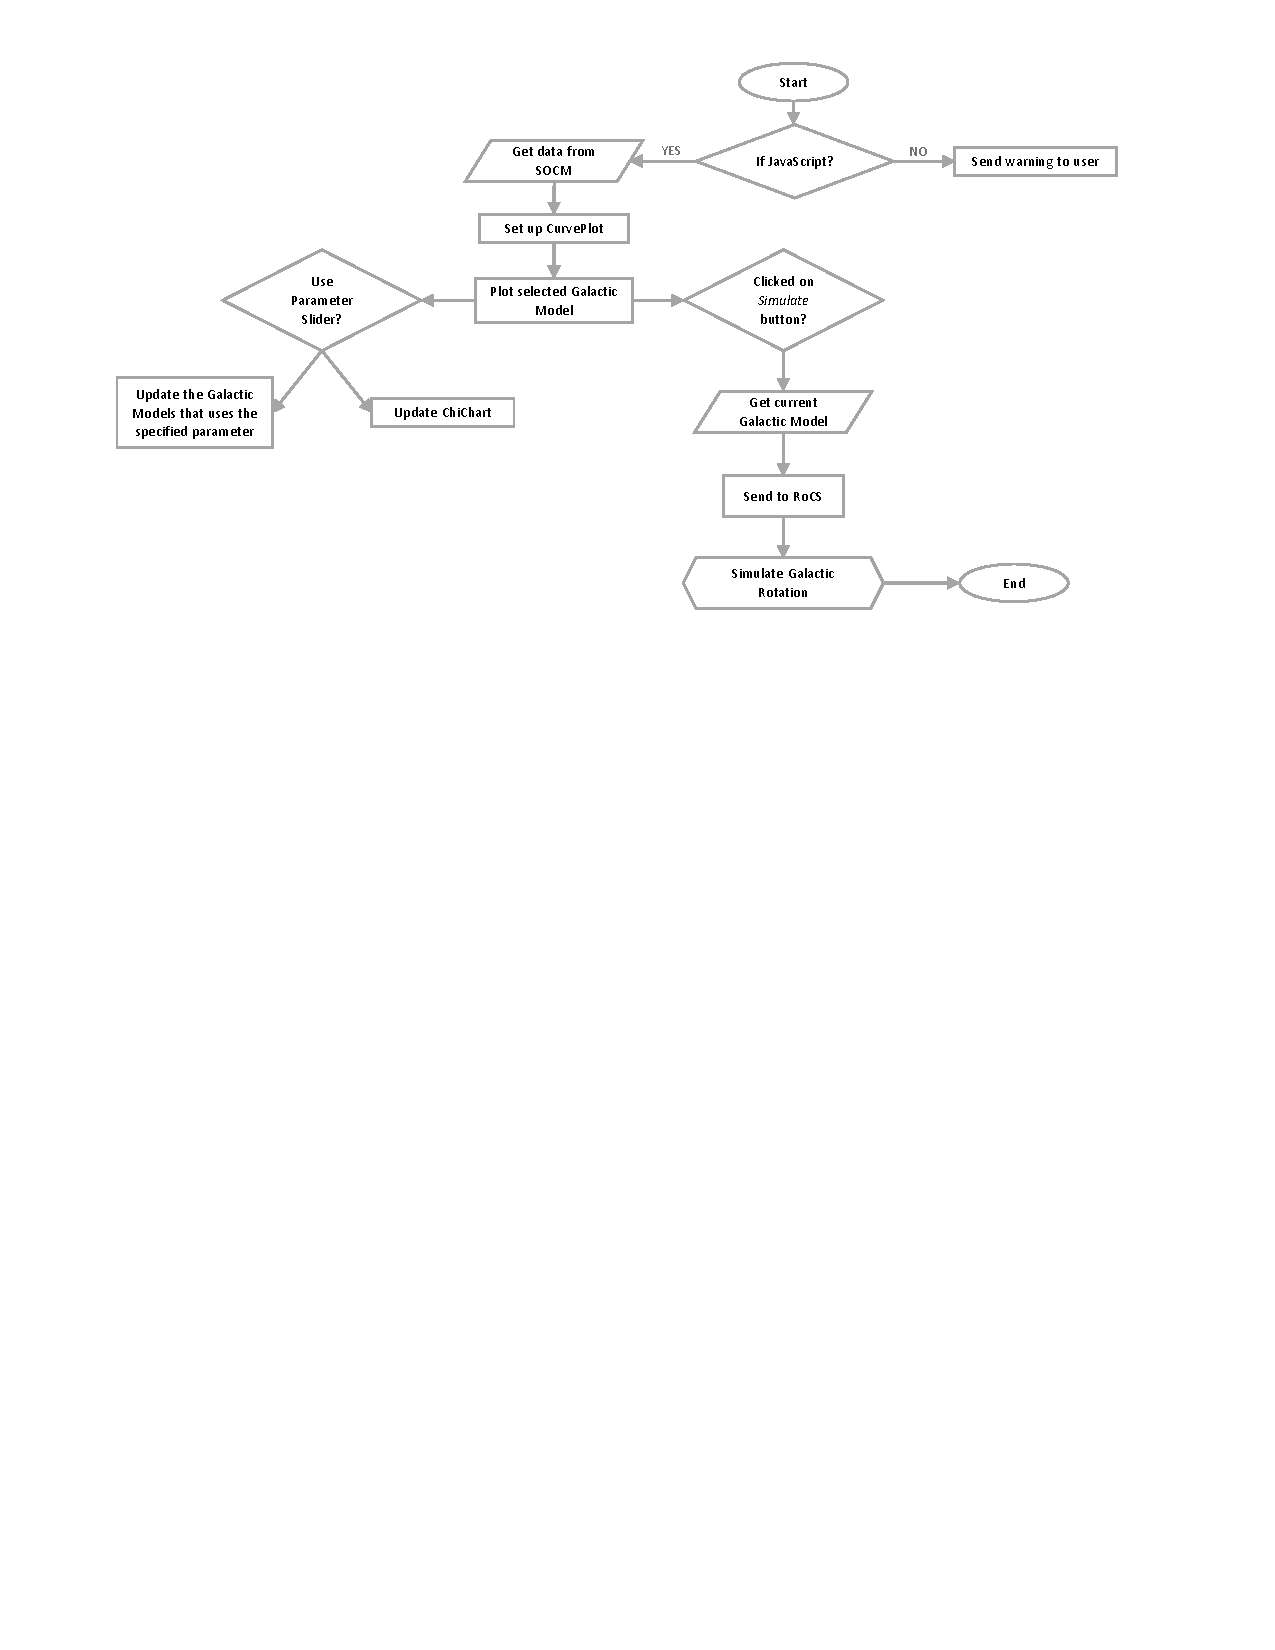
\includepdf[clip,trim=0mm 10cm 0mm 0mm,pagecommand=\subsection{Architectural Design}]{architectural_design.pdf}

% Decomposition Description
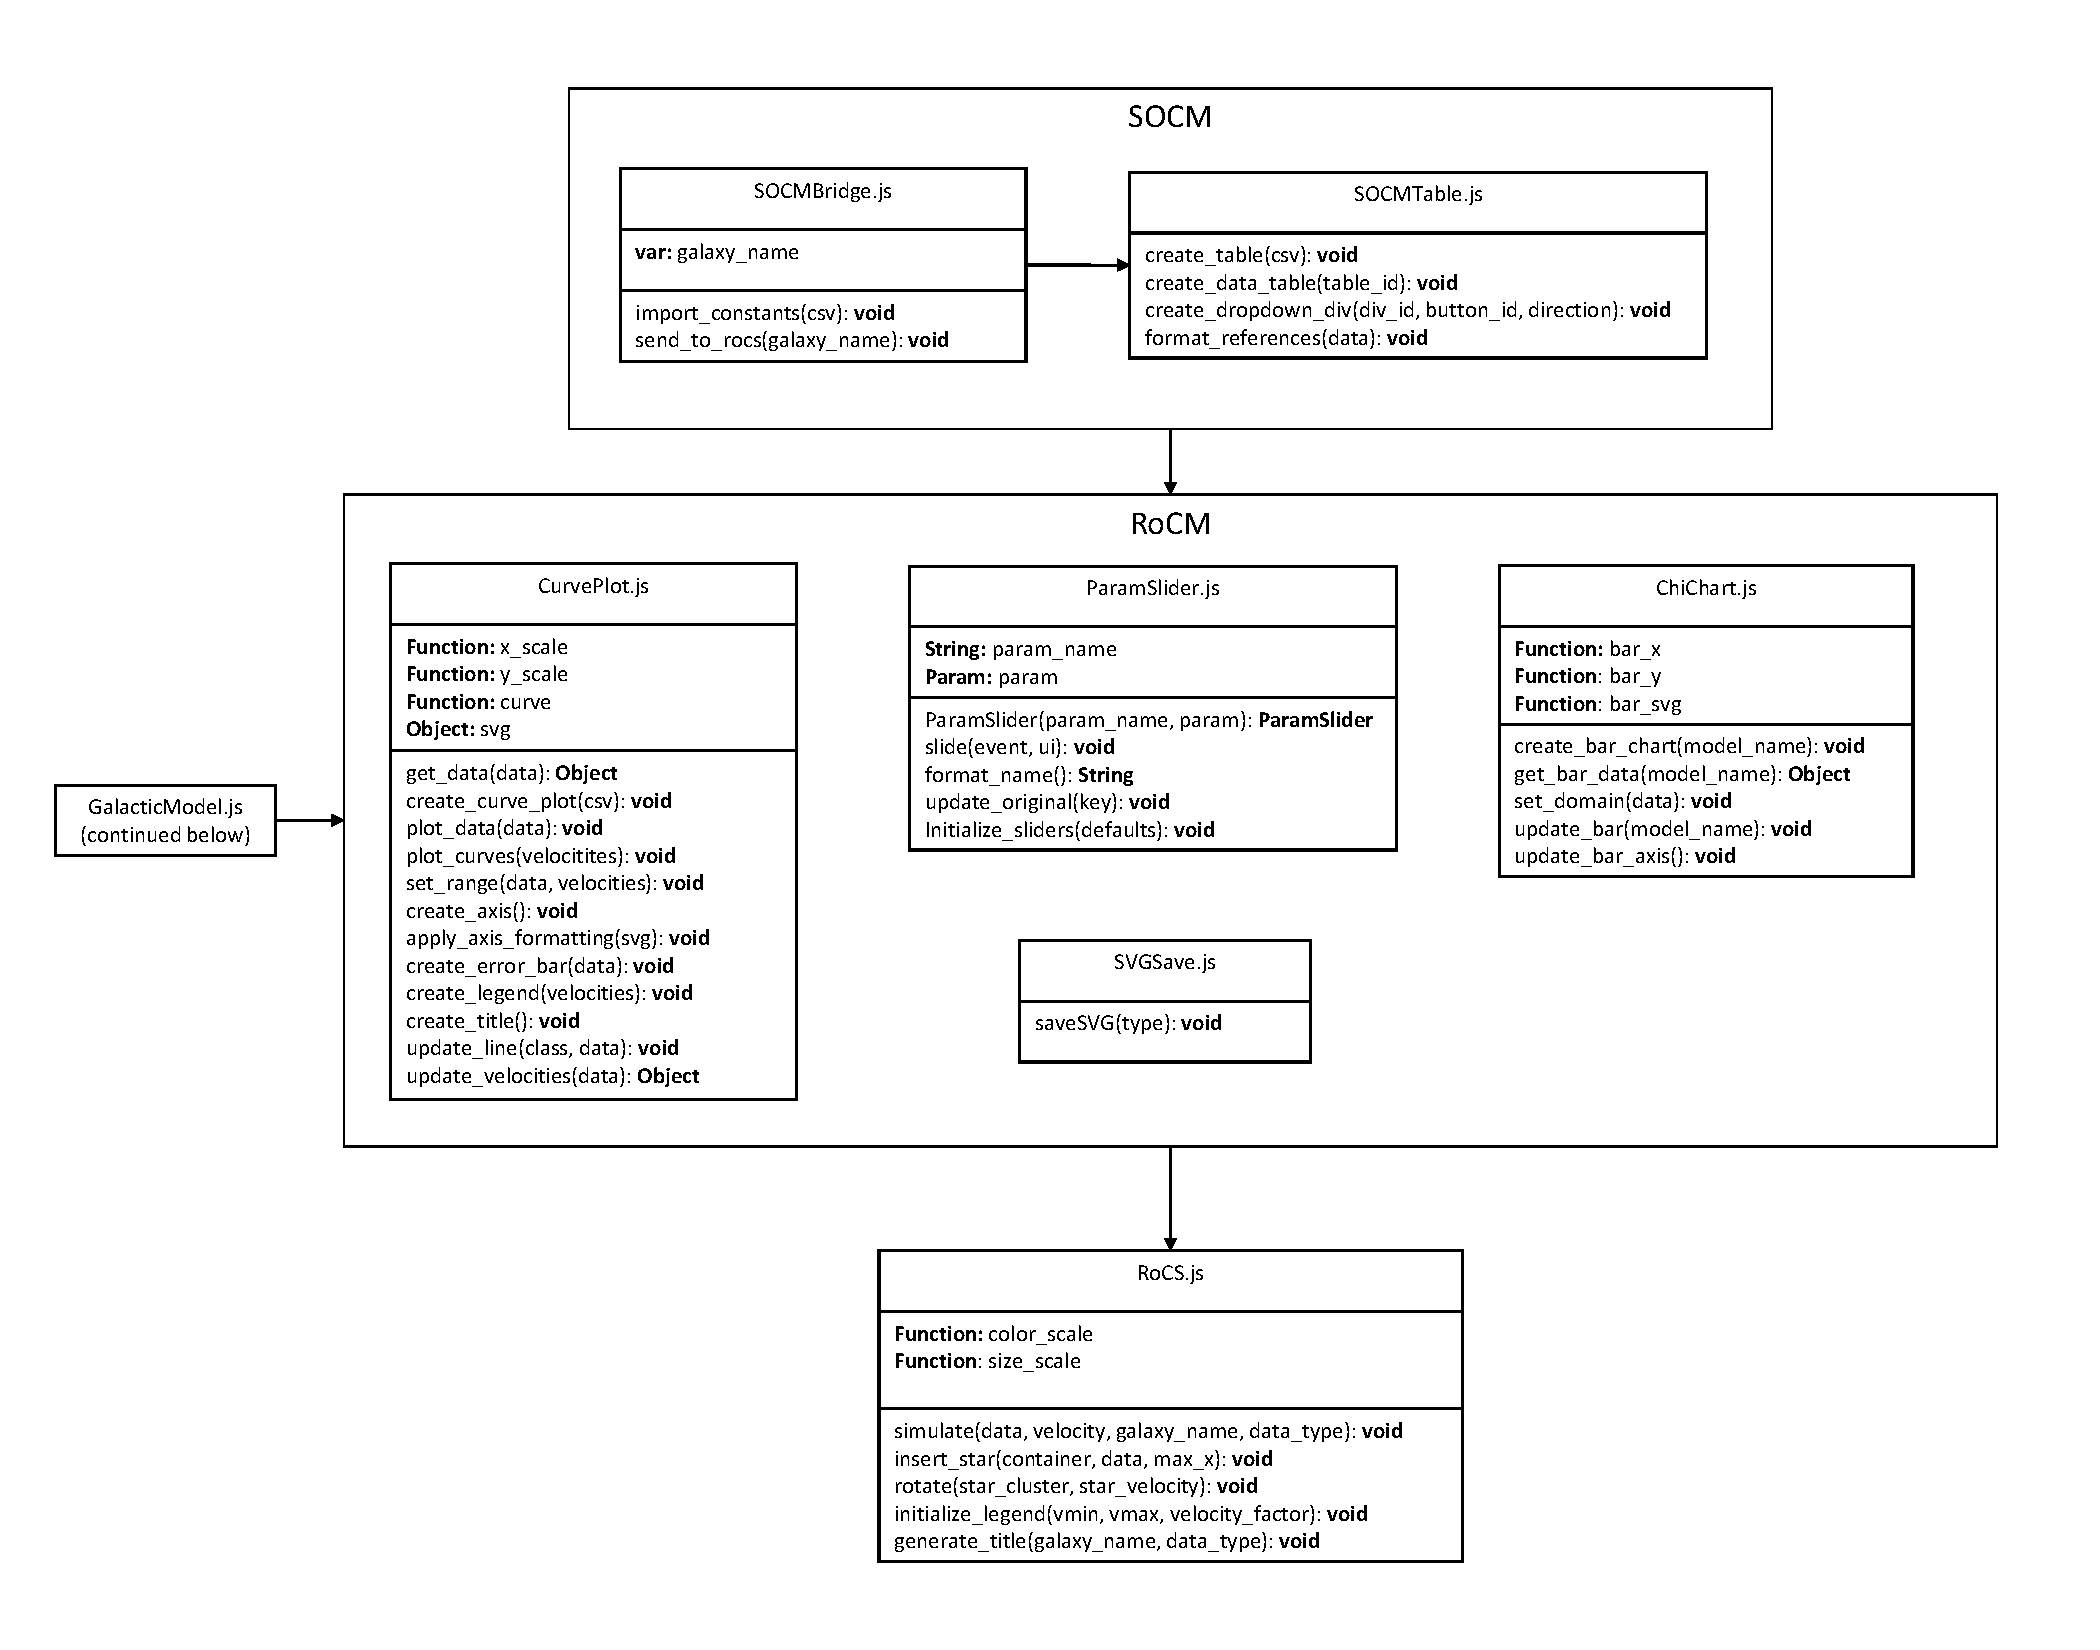
\includepdf[scale=1,pagecommand=\subsection{Decomposition Description}]{decomposition_description_SOCMRoCMRoCS.pdf}
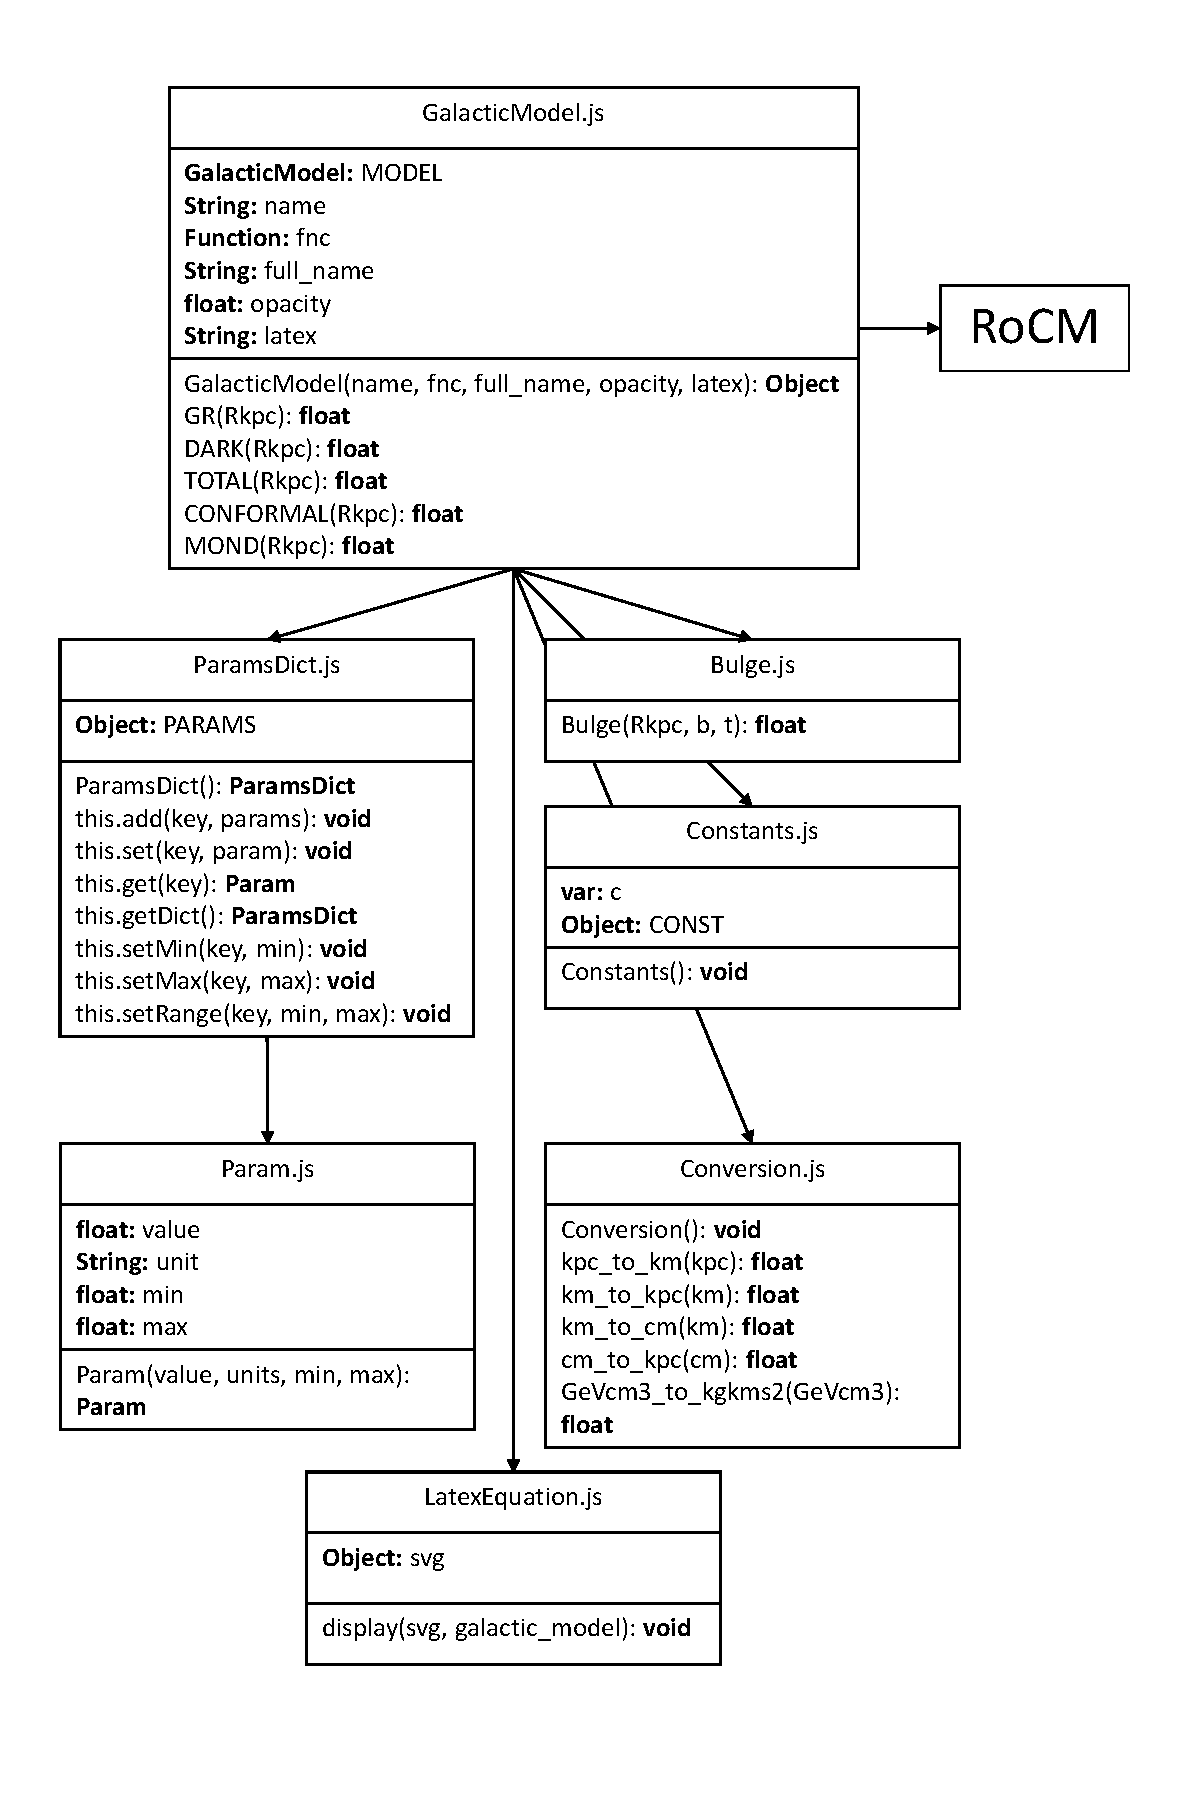
\includepdf[scale=0.75,pagecommand=\subsection{Decomposition Description Continued...}]{decomposition_description_GalacticModel.pdf}

\subsection{Design Rationale}
The design is highly modular. The justification for this is in case other features need to be implemented into RoCM or RoCS. The data retrieval portion of RoCM will be handled by SOCM (and SOCMBridge for data parsing). Splitting up the plotting functions with CurvePlot.js and ChiChart.js will encapsulate the D3.js plotting functionality. Each model will be their own GalacticModel.js, with their own implemented velocity function. When using the global PARAMS object from the ParamsDict.js, the user will be able to use the parameters that come from SOCM within their custom galactic models.

\section{Data Design}
\textit{***See SOCM Software Requirements Specification***}

\section{Component Design}
\subsection{SOCMBridge}
This component will take care of all data transfer from SOCM. The data will be formatted by the specified functionalities (for example: CurvePlot will format the incoming data to plot using D3.js).


\subsection{SOCMTable}
The formatted drop-down table generation will happen within this component. It will receive it's data from SOCMBridge, and create a dynamic table accordingly.

\subsection{CurvePlot}
This component will handle all D3.js plotting of the rotation curves. It comprises of two scale function objects for conversion from a value on a plot, to an screen coordinate. The curve function object will define the shape and inputs of the velocity curve. The svg object will be used throughout in order to draw the svg elements onto an HTML svg tag. The processing of data coming from SOCM will be handled in the get\_data(data) function. Each component of the graph will be generated within their own function (Ex: legend, axes, title, etc.). Update functions for the velocity curves will be provided.

\subsection{ParamSlider}
The defined object, ParamSlider, will have two class variables, a string of the parameter name, and a Param object. The slider has a dynamic slide function which only updates the galactic models that use the changed parameter. 

\subsection{ChiChart}
This component will generate and update the $\chi^2$ statistical testing chart with the current model vs. the observed data. The $\chi^2$ test is formulated by: $\frac{(O - E)^2}{E}$ where $O$ is the observed data and $E$ is the expected result from the model.


\subsection{SVGSave}
This component will take care of converting the CurvePlot svg element into a downloadable format and save it as an SVG file. The importance of a Scalable Vector Graphic file is due to the loss-less format of saving the image as a set of object vectors as opposed to individual pixels.

\subsection{GalacticModel}
The GalacticModel object will contain all of the equations for modeling a galaxy. The object has member variables of the model's name, the equation function (in the form of v(R)), the full formatted model name (for the CurvePlot legend), the line opacity, and the \LaTeX \- equation. Four models will be included: General Relativity (GR), $\Lambda$-Cold Dark Matter (DARK), GR + DARK (TOTAL), Conformal Gravity (CONFORMAL), and Modification of Newtonian Dynamics (MOND). The models can be used throughout the code with the global MODEL object (Ex: cg = MODEL[``CONFORMAL"] will get the Conformal Gravity equation function and can be used by cg(10))

\subsection{Bulge}
This object formulate the bulge contribution of a galactic model. The inner bulge of a galaxy has to be calculated separately from the thin disk.

\subsection{ParamsDict}
The dictionary of Param objects will contain the key (parameter name) and value (Param object) pairs. Additional helper function will be provided in order to implement a standard dictionary. The global PARAMS object can be used in user defined galactic models to access the parameters retrieved from SOCM (Ex: R0 = PARAMS[``R0"] will get the value of R0 from SOCM).


\subsection{Param}
The Param object will define each individual parameter retrieved from SOCM. It has member variables of the float value, the units, and the range of values for the ParamSlider (denoted by min and max). 

\subsection{Constants}
The component will define a global CONST object that contains constant values to be used in any GalacticModel. To access the CONST value, use this syntax CONST[``c"] (this will get the speed of light in kilometers).


\subsection{Conversion}
In order to convert units within RoCM, a custom Conversion object will be provided. Only necessary conversions will be implemented. Conversions from kiloparsecs (kpc), kilometers (km), and centimeters (cm) will be available. For the dark matter model, the conversion from $\frac{GeV}{cm^3}$ to $\frac{kg}{km*s^2}$ will be available.



\subsection{LatexEquation}
This component will handle the conversion from \LaTeX \- code to formatted text via the MathJax library.

\subsection{RoCS}
The Rotation Curve Simulation will handle all rotation visualizations of the galaxy. A color\_scale will be used to display the speed of the star with a color association. The size\_scale function will convert the size of the stars relative to their position from the center (for a better visualization). The simulate function will handle the calls to generate and rotate the stars. 


\section{Human Interface Design}
\subsection{Overview of User Interface}
The GUI will be very minimal, in order to not over complicate the software. A drop-down table will be present to access the SOCM data. From there the user can plot or download that raw data. The Rotation Curve Modeler section will house the CurvePlot functionality and enable the user to \textit{Simulate} the galaxy's rotation or \textit{Save to SVG} the SVG element of the graph. A parameter table will be included to show the current selected galaxy's parameters.

The Sliders section will contains the parameter sliders and the ChiChart. The sliders will be created dynamically by the user, with an additional \textbf{+} button. 

The \LaTeX \- equation section of the web page will show the individual equations for each galactic model. 

Lastly, the About section of the web page will contain information of each component and a tutorial for users on how to operate the software.

For the Rotation Curve Simulation web page, the simulated galactic rotation will be centered with a color scale or the star velocities. A slider for the speed of the spin will enable the user to set the rotation speed accordingly.

\subsection{Screen Images}
\subsubsection{Scholarly Observed Celestial Measurements Table (SOCM Table)}
\begin{adjustwidth}{-2cm}{0pt}
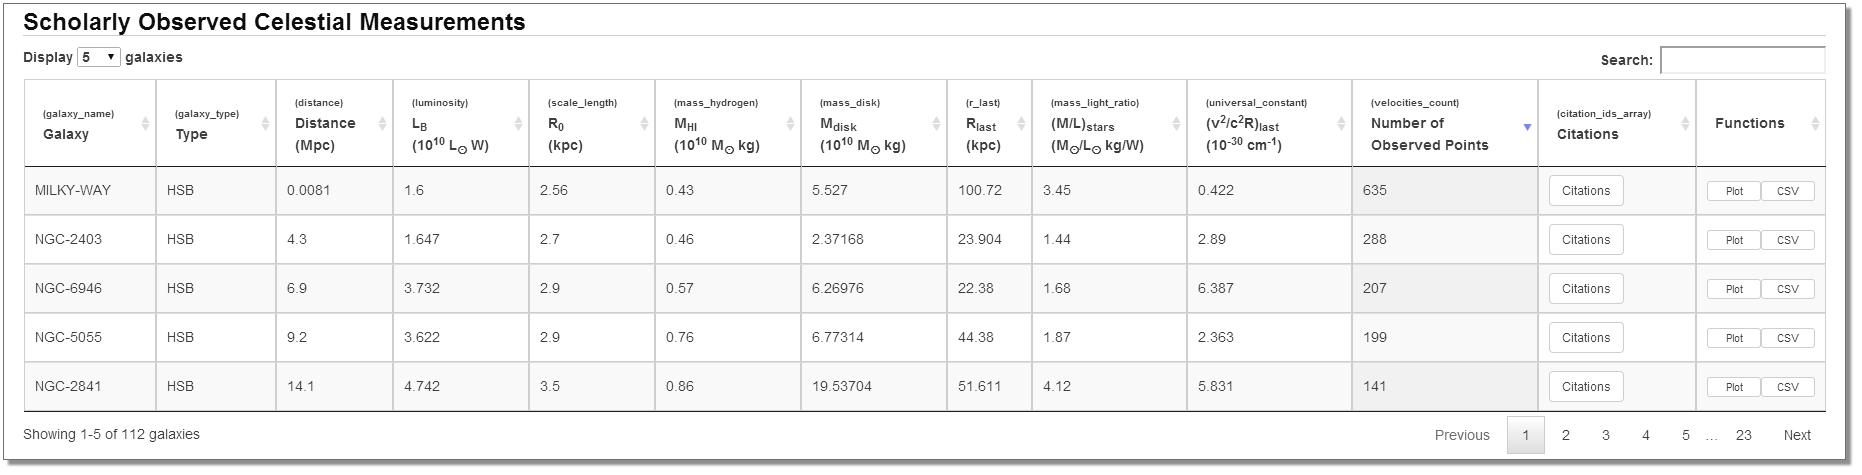
\includegraphics[scale=0.5]{gui/socmtable.png}
\end{adjustwidth}

\subsubsection{Rotation Curve Modeler (RoCM) Web Page}
\begin{adjustwidth}{-2cm}{0pt}
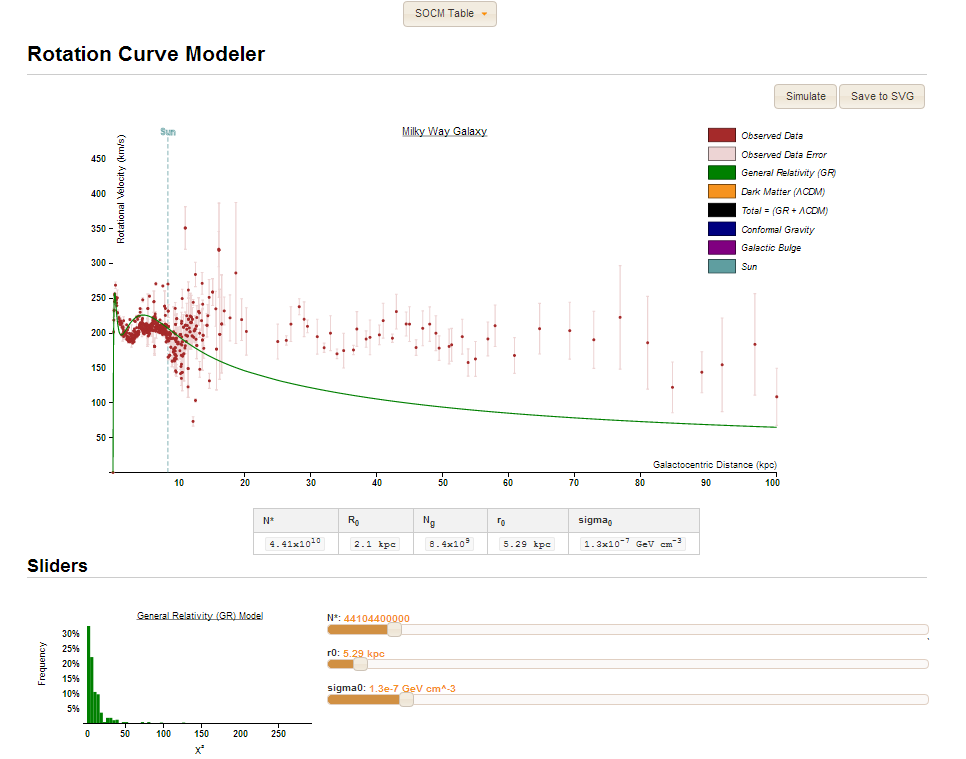
\includegraphics[scale=0.8]{gui/rocm1.png}
\end{adjustwidth}

\subsubsection{Latex Equation Viewer}
\begin{adjustwidth}{-2cm}{0pt}
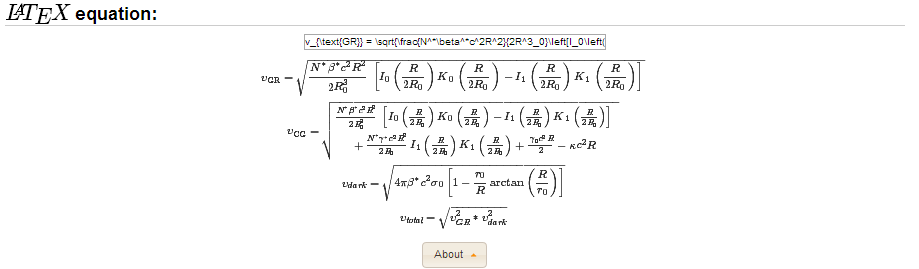
\includegraphics[scale=0.8]{gui/latex.png}
\end{adjustwidth}

\subsubsection{Rotation Curve Simulation (RoCS) Web Page}
\begin{center}
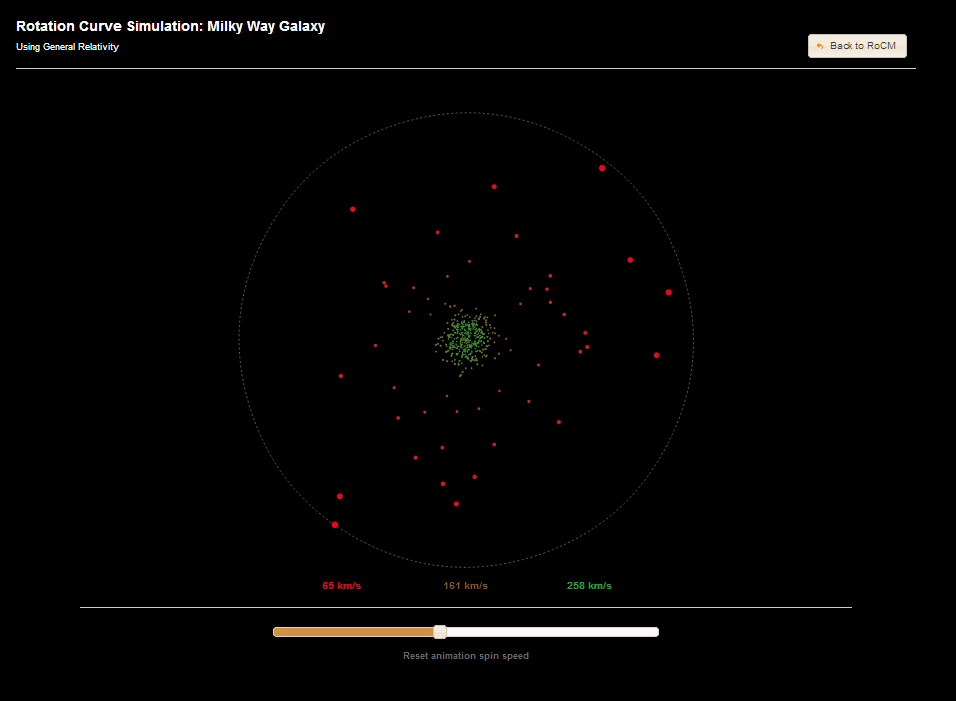
\includegraphics[scale=0.5]{gui/rocs.png}
\end{center}

\end{document}